\chapter{E-Mail Client configuration}
After you set up your secure email server you might want to configure your e-mail client.

The mailserver is only accessible through imaps and requires a TLS certificate for authentication.
Therefor you need to set up your mail client with the appropriate configuration.

At the moment there is only one example for \enquote{Mail on macOS Mojave}.

\section{Mail on macOS Mojave}
\subsection{Mail server config}
\begin{figure}[H]
        \centering
        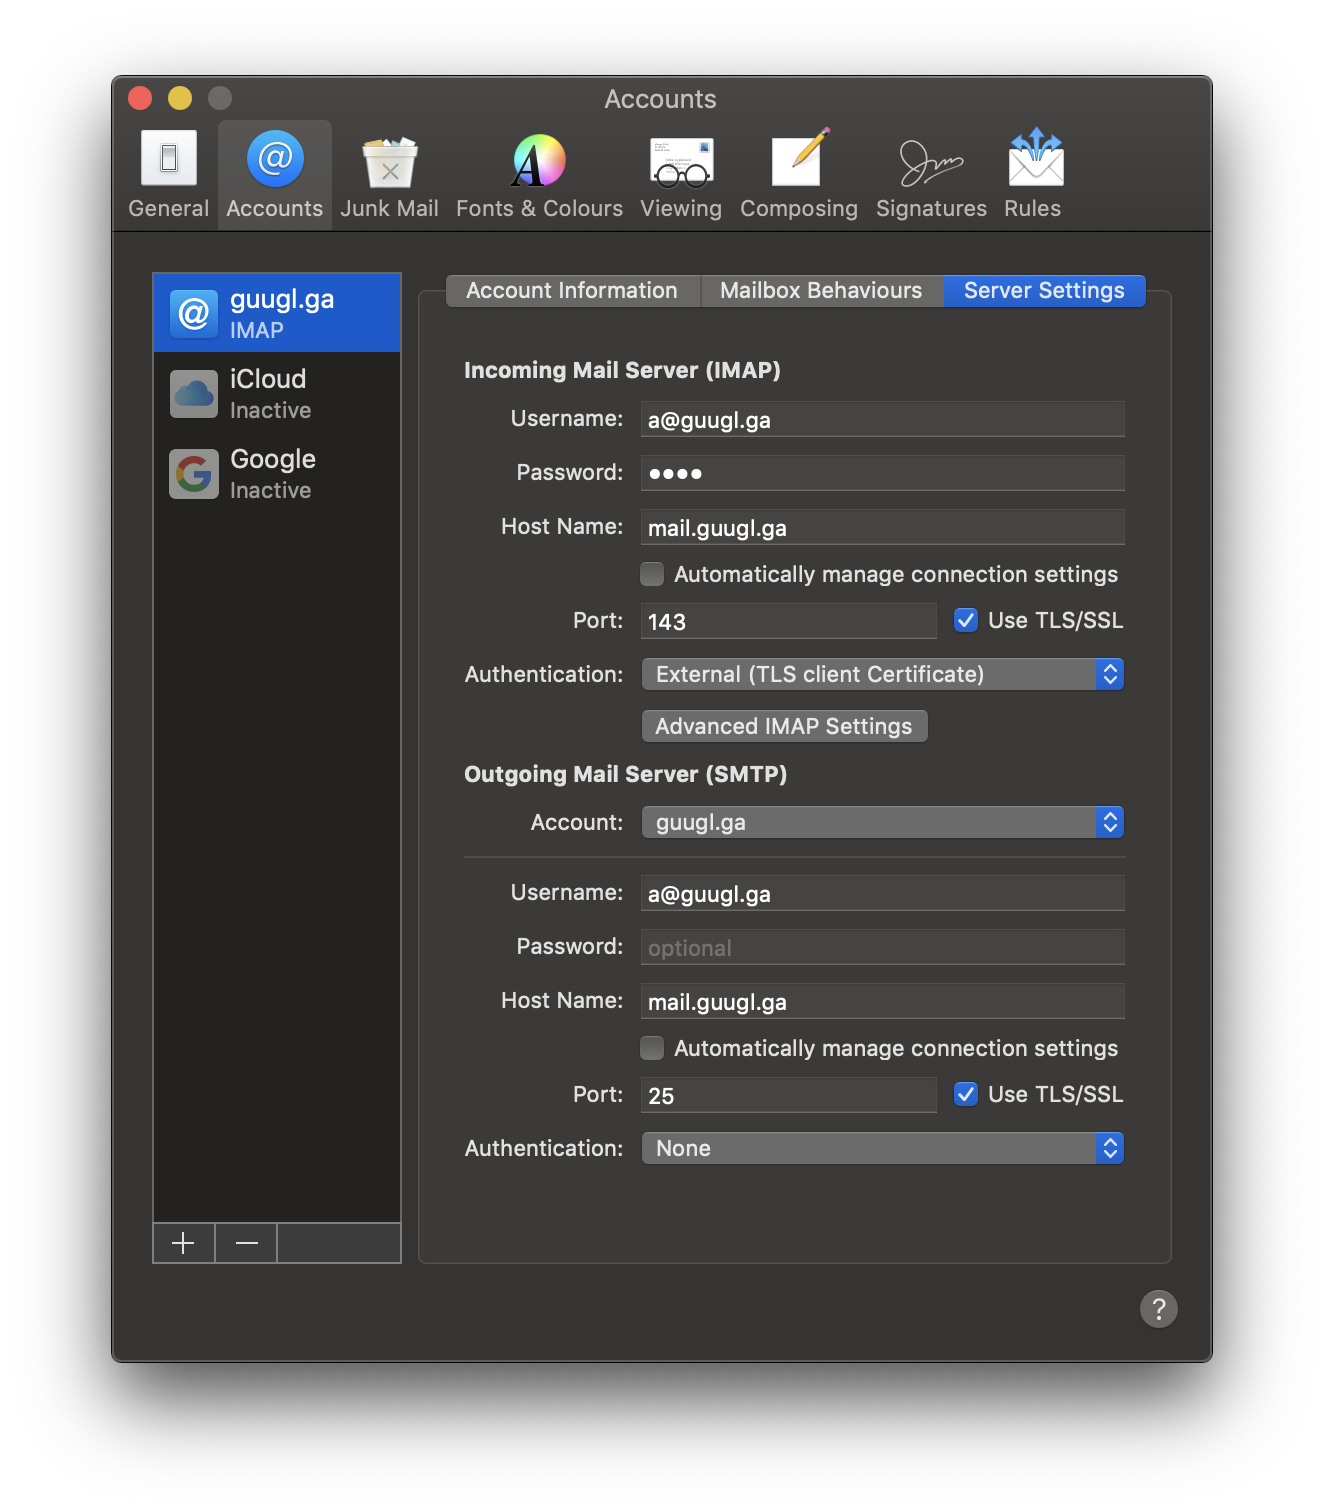
\includegraphics[width=0.8\linewidth]{pics/email_client_config_servers}
        \label{fig:mailserversetting}
                \caption{Mail server config}
\end{figure}

\subsection{Mail SMTP settings}
\begin{figure}[H]
        \centering
        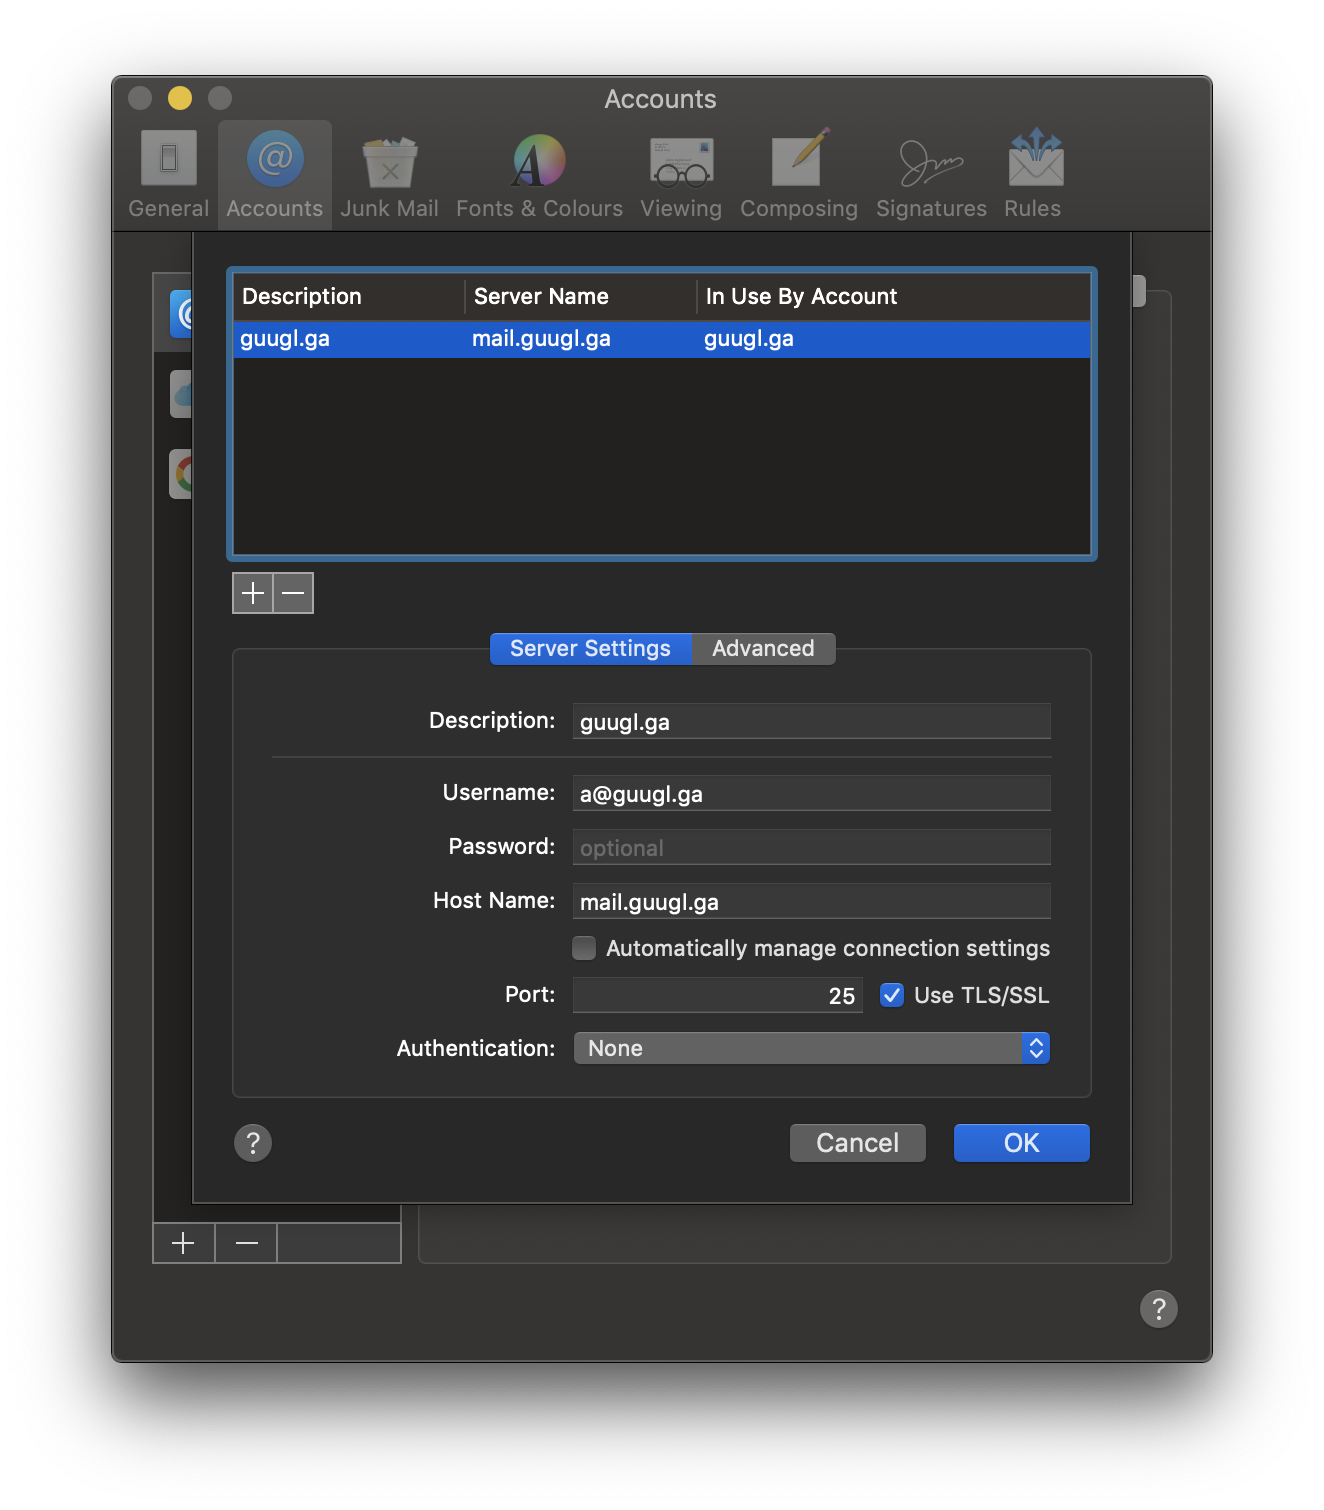
\includegraphics[width=0.8\linewidth]{pics/email_client_SMTP_server_settings}
        \label{fig:mailsmtpsetting}
                \caption{Mail SMTP settings}
\end{figure}

\subsection{Mail IMAP TLS setting}
\begin{figure}[H]
        \centering
        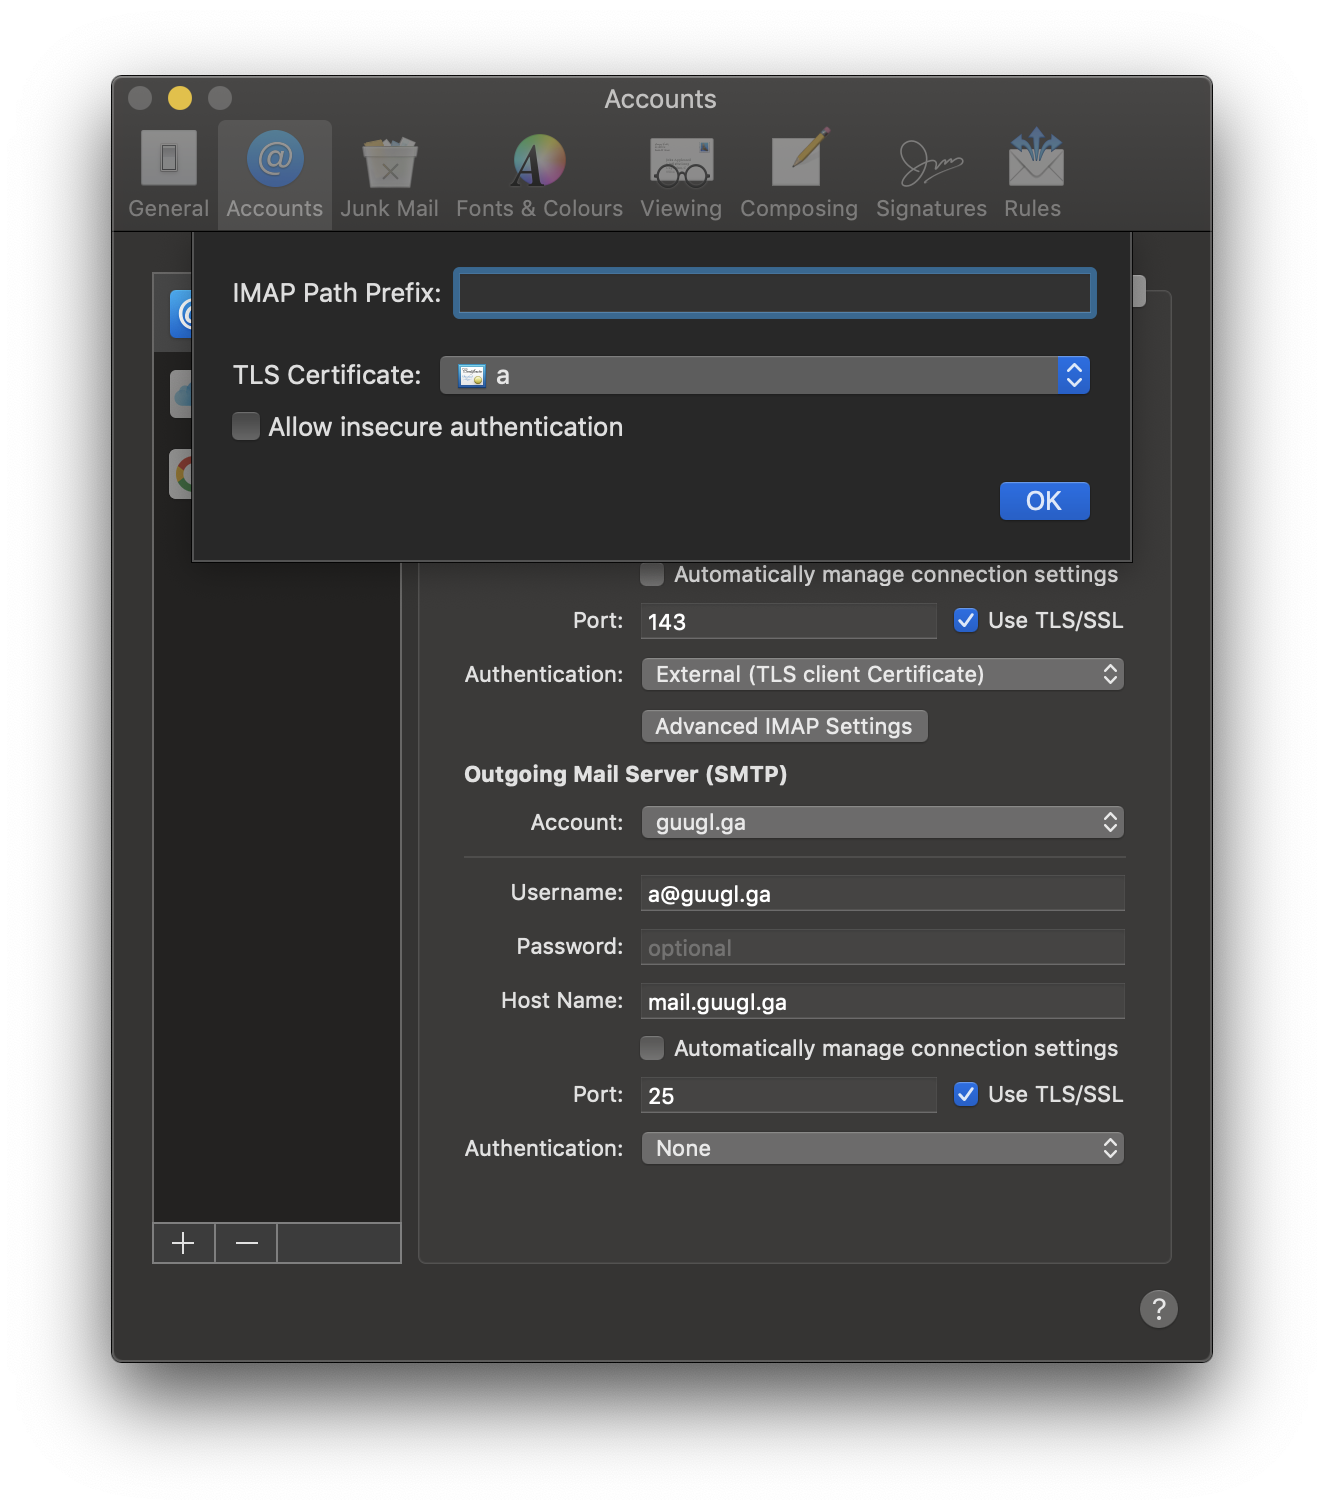
\includegraphics[width=0.8\linewidth]{pics/email_client_IMAP_TLS_settings}
        \label{fig:mailimaptlssetting}
                \caption{Mail IMAP TLS setting}
\end{figure}
